While the described extensions we made to SMACK enable its usage on many Rust
programs, some work remains.
%
First, SMACK currently does not precisely model virtual function tables
generated by a pointer to a structure which implements a trait (i.e., dynamic
polymorphism).
%
We will work towards supporting virtual function tables.
%
Second, Rust programs extensively rely on its standard libraries.
%
While we implemented models for the most common ones, such as \texttt{Vec}, we
plan to model a more substantial subset in the future.
%
% many of the function calls made by Rust
%libraries, e.g., those made by the \texttt{Vec} class, are opaque to SMACK.
%This necessitates the modeling of Rust's libraries rather than relying on
%their definitions. By changing the memory functions used in the Rust libraries
%and a MIR plugin, SMACK should be able handle to handle Rust's library code as
%well.  % We believe aliasing of structures as integer types can be prevented
%by % using plugins for the Rust compiler, particularly through a MIR %
%\cite{mir} plugin, removing the need to define structures such that % they are
%larger than a machine word. A project is currently underway % to fully support
%C++\marek{Citation needed} in SMACK which will form % the basis for supporting
%full dynamic polymorphism. Further % modification to the Rust compiler should
%allow SMACK to control the % manner in which dynamic memory is handled,
%removing the necessity of % modeling Rust's libraries, and instead rely purely
%on their stated % semantics.
%
An additional feature we plan to add is checking of unsafe pointers to ensure
they obey the semantics of the Rust's borrow system.
%
Such pointers typically come from external functions.
%
Since Rust enables legacy code to be used within a project, this feature will
enable developers to verify their wrappers adhere to the Rust's aliasing
semantics.

% \begin{figure}[tb] 
%   % \begin{subfigure}[t]{.6\textwidth}
%   \begin{minipage}[t]{.55\textwidth}
%   \lstset{language=rust,escapechar=|,basicstyle=\footnotesize\ttfamily}
% \begin{lstlisting}
% #[macro_use] mod smack; use smack::*;
% extern{fn fib_c(n:u64)->u64;}|\label{code:cextern}|
% fn fib(x: usize, cache:&mut Vec<u64>){|\label{code:fib_start}|
%   for i in 2..x+1 as usize{|\label{code:iterator}|
%     cache[i]=cache[i-1]+cache[i-2];|\label{code:overflow}|
%  }
% }|\label{code:fib_end}|
% fn main(){
%   let n=5u64.nondet();|\label{code:nondet}|
%   assume!(n > 2);|\label{code:assume}|
%   let mut cache=vec![0; n+1];|\label{code:mkvec}|
%   cache[0]=0;|\label{code:vectoridx}|
%   cache[1]=1;
%   fib(n, &mut cache);|\label{code:fncall}|
%   let c_result=unsafe{fib_c(n)};|\label{code:ffi}|
%   assert!(cache[n]==c_result);|\label{code:assert}|
% }
% \end{lstlisting}
%   \end{minipage}
%   % \begin{subfigure}[t]{.4\textwidth}
%   \begin{minipage}[t]{.4\textwidth}
%   \lstset{language=c,basicstyle=\footnotesize\ttfamily}
%     \begin{lstlisting}
% typedef unsigned long ul;
% ul fib_c(ul x) {
%   ul a = 0, b = 1;
%   for (ul i=0; i<x-1; i++) {
%     ul tmp = a;
%     a = b;
%     b = a + tmp;
%   }
%   return b;
% }
% \end{lstlisting}
% \end{minipage}
% %\caption{Example program showing Rust features we support.  It checks the Rust
% %implementation of the Fibonacci function (left) against the
% %corresponding C implementation (right).}
% \caption{Rust program that checks the equivalence between the Rust (\texttt{fib}) and C (\texttt{fib\_c}) implementations of the Fibonacci function.}
% \label{fig:crossfib}
% \end{figure}


% \begin{figure}[tb]
%   \centering
%   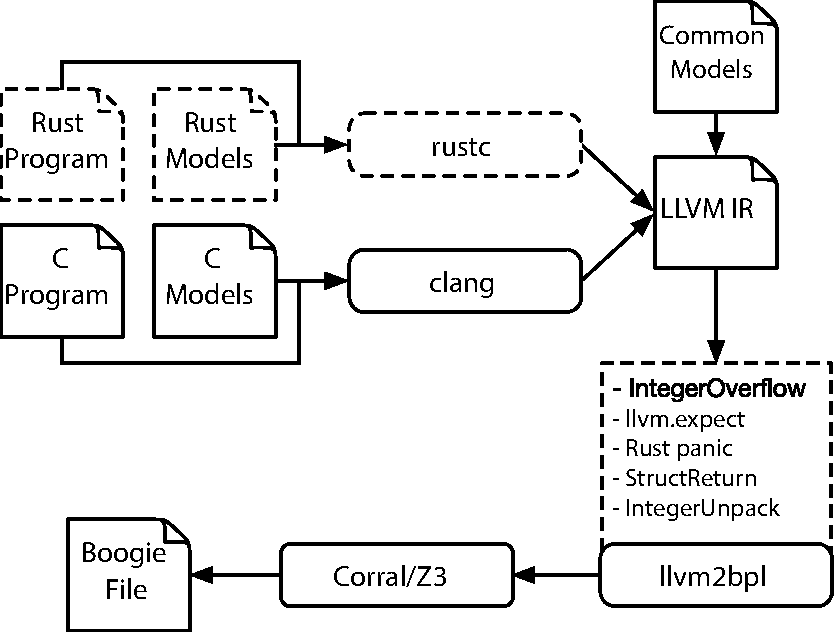
\includegraphics[width=0.99\textwidth]{chap2/figures/RustSmack.pdf}
%   \caption{SMACK extensions for Rust.}
%   \label{fig:atvatoolflow}
% \end{figure}

% \begin{figure}[tb]\lstset{language=boogie,basicstyle=\scriptsize\ttfamily}
% \begin{lstlisting}
% // %x = call {i8,i1} @llvm.uadd.with.overflow.i8(i8 %a,i8 %b)
% $a2 := $zext.i8.i16($a);
% $b2 := $zext.i8.i16($b);
% $x2 := $add.i16($a2, $b2);
% $x  := $trunc.i16.i8($x2);
% $flag  := $ugt.i16($x2, 255);
% assert !$flag;
% \end{lstlisting}
% \caption{Translation of an unsigned 8-bit checked-addition intrinsic.}
% \label{fig:overflow}
% \end{figure}

% \begin{table}[tb]
% \begin{center}
% \label{tab:benchmarks}
% \begin{tabular}{|c|c|c|c|}
% \hline
% \textbf{Benchmark category} & \textbf{\#Files} & \textbf{LOC} & \textbf{Features demonstrated} \\
% \hline
% \hline
% functions and recursion & 8 & 153 & Function calls, closures, and recursion \\
% generics & 6 & 55 & Generic functions, structures, and traits \\
% ifc  & 4 & 214 & Information flow control example \\
% loops & 4 & 35 & Range-based for loops \\
% %other & 4 & Use of nondeterministic values \\
% ops & 12 & 171 & Basic operations, overflows \\
% %recursion & 4 & Recursive functions \\
% structures & 4 & 76 & Creation, passing, and returning of structures \\
% vector & 6 & 88 & Dynamic memory management \\
% cross-language & 4 & 48 & Combining Rust and C \\
% \hline
% \end{tabular}
% \end{center}
% \caption{Summary of the benchmark suite we developed.}
% \end{table}